\section{Results}
After having translated the datasets into more workable and query-able formats, which on its own is quite a result already, the KPIs could be checked for their compliance. By writing and querying rather complex XQueries, we were able to check the compliance of the KPIs. Table \ref{table:kpiAndExploration} on page \pageref{table:kpiAndExploration} displays the obtained results for the KPI checks and the Exploration.

For both educational years we have calculated the values for the KPIs. The first KPI says that a student should have a minimum of 4 contact hours on a day (if they have any). In the first year the KPI has been met 75.06\% of the time, the last year 71.04\% of the time. The second KPI describes that a student should have 6 or less contact hours a day, which is met 58.84\% in the first year and 63.07\% in the second year. A couple of KPI cannot easily be measured as a percentage of compliance, and therefore have an absolute count. For example the sixth KPI describes that on Friday there should not be evening classes, which has been violated 269 times in the first year and 99 times in the second year. With these numbers you could still check for trends over the years. KPI nine describes that rooms should have an occupation of at least 70\% during educational weeks, this has been met for just one room in the first year, and zero rooms in the second year. For results of the other KPIs see Table \ref{table:kpiAndExploration}  on page \pageref{table:kpiAndExploration}.

Not only did we check the KPIs given by the University itself but we also came up with a few other analyses to point out some interesting discoveries in the data sets. As mentioned before, these results are displayed on the website \url{http://wiefferink.me/TimeTabling}. The statistics we came up with are results per quartile, this means a statistic has been counted for each quartile in the two studied years.

From the KPIs we learned that ideally a student has 4-6 hours, so we made this visual by splitting it in a couple categories and then display them in a stacked bar graph. Figure \ref{fig:dayLengtsStudents} shows these results, the activity count is seen in the vertical axis, the quartiles in the horizontal axis. With this graph the distribution between the chosen categories can be seen. The same analysis has been executed for teachers, which can be found on the website.

\begin{figure}[!h]
	\centering
	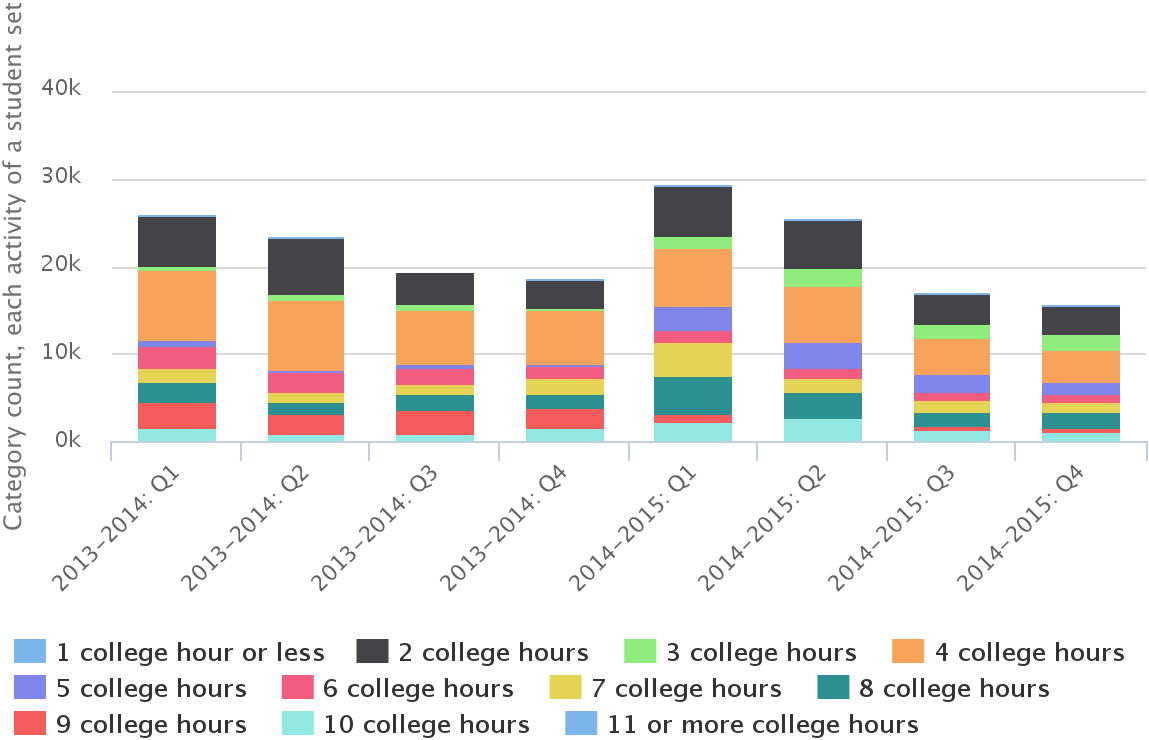
\includegraphics[width=80mm]{dayLengthsStudents.png}
	\caption{Day lengths for students}
	\label{fig:dayLengtsStudents}
\end{figure}

The next statistic is about the wasted hours of teachers and students, which was also in interest by the KPIs. The bar graph in Figure \ref{fig:wastedHours} shows the distribution between useful and 'wasted' hours.

\begin{figure}[!h]
	\centering
	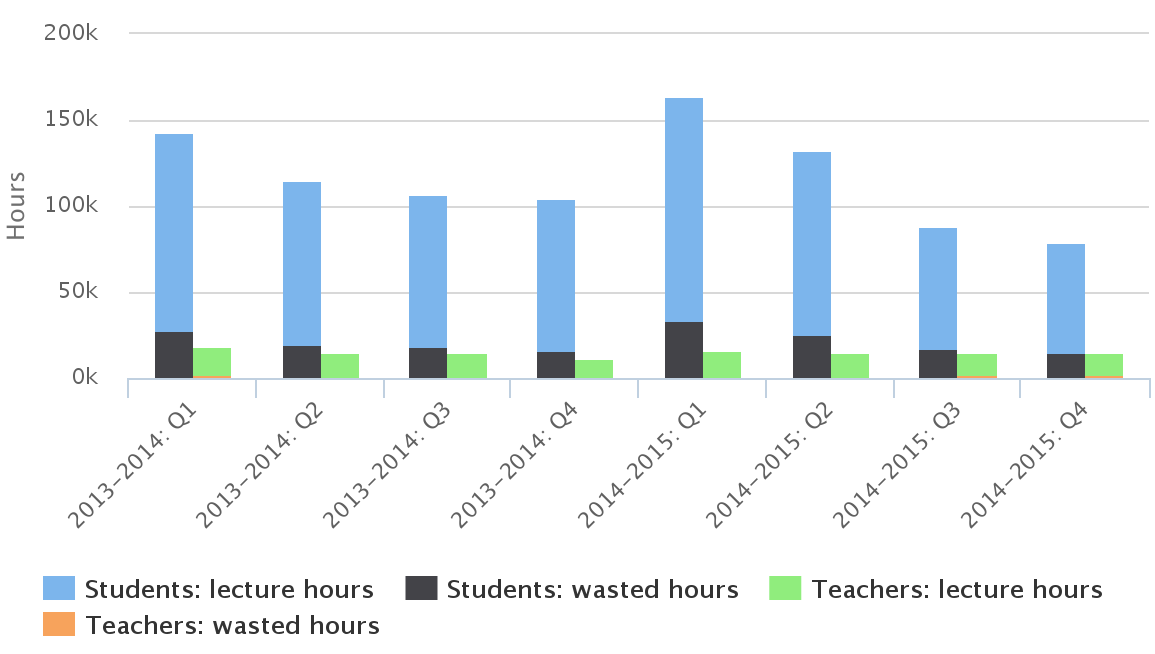
\includegraphics[width=80mm]{wastedHours.png}
	\caption{Wasted hours for students and teachers}
	\label{fig:wastedHours}
\end{figure}

Furthermore we investigated the distribution of lecture types among activities, Figure \ref{fig:lectureTypes} shows the result. For each quartile the number of activities of a certain lecture type can be seen.

\begin{figure}[!h]
	\centering
	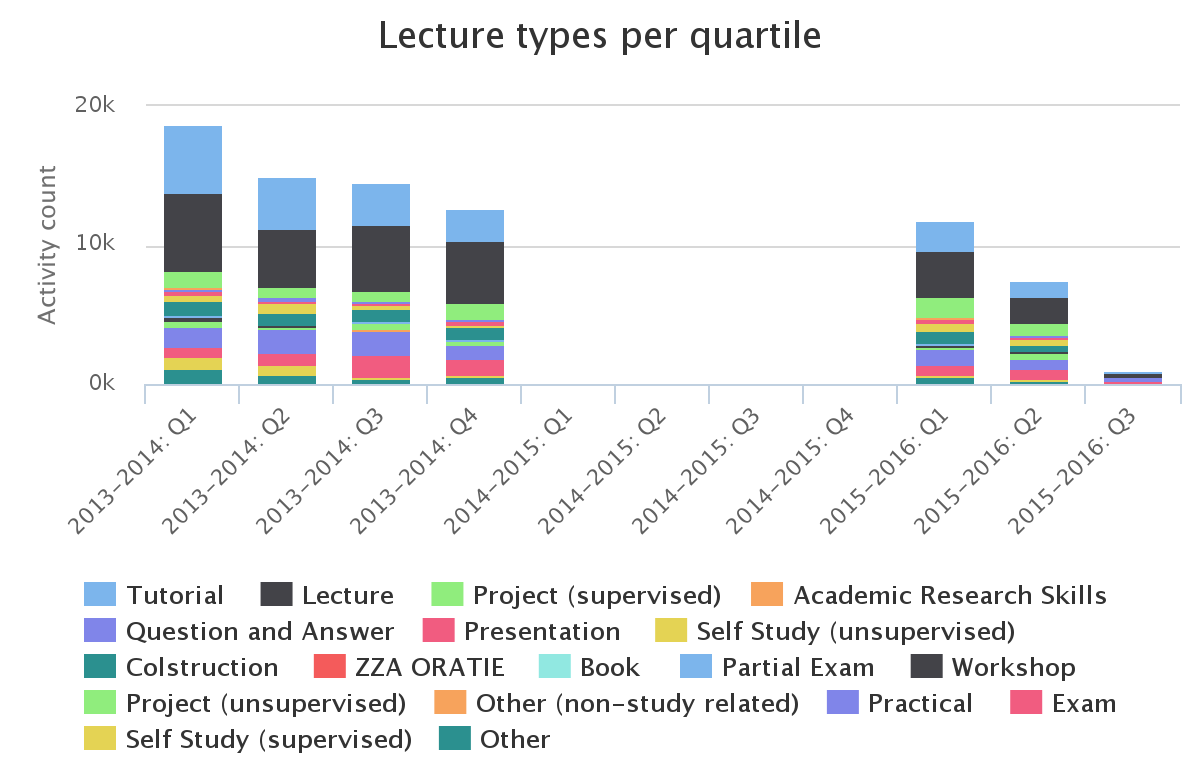
\includegraphics[width=80mm]{lectureTypes.png}
	\caption{Lecture types}
	\label{fig:lectureTypes}
\end{figure}

As last we have counted the number of teachers, student sets and activities per quartile, these could be used to correct the other data or give insight in the activity on the university.
